% Chapter 7

\chapter{Background Processes} % Chapter title

\label{ch:background_processes} 

%----------------------------------------------------------------------------------------

This analysis is fundamentally a search for Supersymmetry in events with two leptons whose invariant mass is consistent with a Z boson. Additional event selections are made to reduce Standard Model processes relative to potential Supersymmetric processes, defined by simplified models discussed in \autoref{sec:simplified_models}. Supersymmetric events typically have large amounts of \MET, \HT (the scalar sum of the \pT of objects in the event), and many jets. All of these features can help isolate these events from backgrounds. To understand what cuts would optimize the sensitivity of the search, it is essential to first understand what these Standard Model backgrounds are. 

\begin{centering}
\begin{figure}[bth]
\myfloatalign
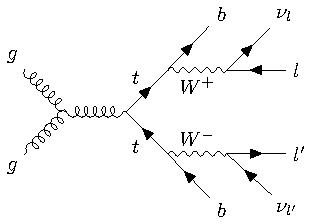
\includegraphics[width=.70\linewidth]{feynman/ttbar.pdf}
\caption{An example Feynman diagram of \ttbar production and decay.}
\label{fig:ttbar}
\end{figure}
\end{centering}

\paragraph{\ttbar} is the largest background for this search. \autoref{fig:ttbar} shows an example of this process, which can decay to many jets, leptons, and neutrinos, which are seen in the detector as \MET. Thus, \ttbar naturally has high \MET and \HT, jets, and leptons from two different W boson decays, which may coincidentally form an invariant mass on the Z peak. These events are very difficult to separate from potential signals, though keeping the mass window small and increasing \MET and \HT above the typical values for \ttbar events can help reduce them.

\begin{centering}
\begin{figure}[bth]
\myfloatalign
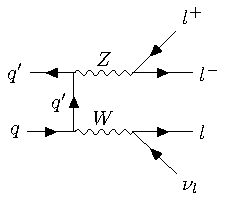
\includegraphics[width=.70\linewidth]{feynman/diboson.pdf}
\caption{An example Feynman diagram of the production and decay of a WZ event.}
\label{fig:diboson}
\end{figure}
\end{centering}

\paragraph{diboson} production is the next leading background. These events can contain real Z bosons and will peak on-Z like a signal. In addition, in events like \autoref{fig:diboson}, an additional W boson can decay to another lepton and a neutrino, providing \MET. The pictured process can occur with associated jets, but at reduced rates, so adding a jet requirement to the signal region can help reduce these events. If the W boson in this diagram instead decayed to two jets, there would be no true \MET from a neutrino, so a \MET cut in conjunction with a jet cut is very effective in reducing the total diboson background. 

\section{Monte Carlo Samples} 